\documentclass[letter]{article}

\usepackage{ijcai15}
\usepackage{times}

\usepackage{eurosym}
\usepackage{hyperref}		% clickable references

\usepackage{apacite}            % APA style citations
\usepackage{apacdoc}

\usepackage{amsmath,amssymb}	% math structures and symbols
\usepackage{graphicx}		% including of graphics files in various formats
\usepackage{amsfonts}
\usepackage{dialogue}
\usepackage{placeins}
\usepackage{tikz}
\usetikzlibrary{positioning,backgrounds,fit,arrows,shapes,shadows}
\usetikzlibrary{shapes.multipart}
\usepackage{wrapfig}
\usepackage{enumitem}
\usepackage{framed}

% \hypersetup{hidelinks}

\usepackage[xspace,mla]{ellipsis}

\definecolor{myyellow}{RGB}{242,226,149}
\definecolor{mygreen}{RGB}{144,238,144}
\definecolor{mypink}{RGB}{255,182,193}
\definecolor{myorange}{RGB}{255,165,0}
\definecolor{myblue}{RGB}{0,204,204}

\usepackage{xparse}
\NewDocumentCommand\StickyNote{O{4cm}mmO{4cm}}{%
\begin{tikzpicture}
\node[
drop shadow={
  shadow xshift=2pt,
  shadow yshift=-4pt
},
inner xsep=7pt,
fill=#2,
xslant=-0.05,
yslant=0.05,
inner ysep=10pt
] {\parbox[t][#1][c]{#4}{#3}};
\end{tikzpicture}%
}

\urldef{\mailsa}\path|{j.corneli,s.colton}@gold.ac.uk|
\urldef{\mailsb}\path|a.pease@dundee.co.uk|

\newcommand{\Fw}{{\sf FloWr}}
\newcommand{\dec}[1]{\raisebox{.2ex}{$\star$}#1\raisebox{.2ex}{$\star$}}

\newcommand{\keywords}[1]{\par\addvspace\baselineskip
\noindent\keywordname\enspace\ignorespaces#1}

\begin{document}

% TITLE INFORMATION
\title{Implementing feedback in creative systems}

\author{Joseph Corneli\textsuperscript{1} and Anna Jordanous\textsuperscript{2}\\
\textsuperscript{1} Department of Computing, Goldsmiths College, University of London\\
\textsuperscript{2} School of Computing, University of Kent}

\date{today}

\maketitle

\begin{abstract} 
% First attempt
%% Various social strategies, ranging from Writers Workshops to open
%% source software, pair programming, and design charettes have been
%% developed to exploit emergent effects and to develop new shared
%% language.  We investigate the feasibility of using designs of this
%% sort in multi-agent systems that learn by sharing and discussing
%% partial understandings.  Building on earlier theoretical work, we
%% describe concrete implementation plans and some preliminary results.
\end{abstract}

\section*{\emph{Outline}} \label{sec:outline}

{\small
\begin{enumerate}[start=0,label=\textbf{\arabic*}]
\item \textbf{\emph{Implementing feedback in creative systems: a writers
  workshop approach.}}
\item[] Contributions:
\begin{enumerate}
\item \emph{Introduce} the writers workshop as a model for learning
  from feedback; and
\item \emph{Survey} the aspects of feedback that can be offered, and
  how they can be interpreted; and
\item \emph{Present} a case study on how to implement this, at a level
  that other people could use to implement similar Workshop designs in
  their own creative systems.
\end{enumerate}
\item \textbf{Here is the writers workshop idea.}
\item[] The steps:
\begin{enumerate}
\item A: {\tt presentation}
\item C: {\tt listening}
\item C: {\tt feedback} ({\tt observations}{\tt+}{\tt suggestions})
\item A: {\tt questions}
\item C: {\tt replies}
\item A: {\tt reflections}
\end{enumerate}
\item[] Previous applications:
\begin{enumerate}[label=(\roman*)]
\item We sketched a ``theory of poetics rooted in the making of
  boundary-crossing objects and processes''
\item We ``described a system that can (sometimes) make `highly
  serendipitous' creative advances in computer poetry'' while
  ``drawing attention to theoretical questions related to program
  design in an autonomous programming context.''
\end{enumerate}
\item \textbf{Here we refine the idea and turn it into a general model
  that for incorporating feedback within computational models of the
  creative process.}
\item[] What can feedback be about? \dec{Survey}
\begin{enumerate}
\item Patterns that \emph{match} and any \emph{exceptions}
\item Progress relative to explicit or adduced \emph{exploration}
  (knowledge and accuracy) or \emph{exploitation} (directional,
  task-based) goals.
\item \emph{Quantity}, \emph{Variety}, and \emph{Order} of produced
  objects or behaviours
\item New relationships among produced objects and behaviours drawing
  on a common field of reference
\end{enumerate}
\item[] How can feedback be understood and used? \dec{Survey}
\begin{enumerate}
\item Update knowledge base with new facts (accept statements,
  possibly with provenance)
\item Note similarity to \emph{iterative development}
\item Reflection: describe relationships between produced objects and
  behaviours and feedback
\item Reflection: Higher-order patterns e.g.~new patterns that
  describe the identified exceptions
\end{enumerate}
\item \textbf{As we happened to be working with \Fw\ to model the
  creative process, we will use \Fw\ as a case study to exemplify how
  to implement this writers workshop model to use feedback within
  being creative.}
\item[] What can we give feedback about in this context?
\begin{enumerate}
\item \emph{Population of nodes}: what can they do?  what do we learn when a
  new node is added?
\item \emph{Population of flowcharts}: Simon and Alison have talked
  about ``broken'' flowcharts; this suggests a sort of test-driven
  development framework.
\item \emph{Population of output texts}: how to generate commentary on
  a generated artefact?
\end{enumerate}
\item[] How will the feedback be understood and used?
\begin{enumerate}
\item ?
\item ?
\item Connect commentary on a generated artefact with the code that
  made that artefact.
\end{enumerate}
\item \textbf{Discussion of how this would work more generally in
  computational creativity and perhaps in AI more generally.}
\begin{enumerate}
\item Feedback is the fundamental concept in \emph{cybernetics}.  \dec{Definition?}
\item Feedback about feedback (\&c for higher orders) is relevant to thinking about \emph{learning} and \emph{communication}
\item \emph{Creativity} is often envisaged as cyclical process (e.g.~Dickie's
  art circle, Colton et al.~Iterative
  Development Expression Appreciation).  There are opportunities for
  embedded feedback at each step, and the process itself is ``akin
  to'' a feedback loop.
\end{enumerate}
\item \textbf{Conclusion: we have described a \emph{general} and \emph{computationally feasible} model for learning from feedback.}
\end{enumerate}
}

%\documentclass[letter]{article}
%
%\usepackage{ijcai15}
%\usepackage{times}
%
%\usepackage{eurosym}
%\usepackage{hyperref}		% clickable references
%
%\usepackage{apacite}            % APA style citations
%\usepackage{apacdoc}
%
%\usepackage{amsmath,amssymb}	% math structures and symbols
%\usepackage{graphicx}		% including of graphics files in various formats
%\usepackage{amsfonts}
%\usepackage{dialogue}
%\usepackage{placeins}
%\usepackage{tikz}
%\usetikzlibrary{positioning,backgrounds,fit,arrows,shapes,shadows}
%\usetikzlibrary{shapes.multipart}
%\usepackage{wrapfig}
%\usepackage{enumitem}
%\usepackage{framed}
%
%% \hypersetup{hidelinks}
%
%\usepackage[xspace,mla]{ellipsis}
%
%\definecolor{myyellow}{RGB}{242,226,149}
%\definecolor{mygreen}{RGB}{144,238,144}
%\definecolor{mypink}{RGB}{255,182,193}
%\definecolor{myorange}{RGB}{255,165,0}
%\definecolor{myblue}{RGB}{0,204,204}
%
%\usepackage{xparse}
%\NewDocumentCommand\StickyNote{O{4cm}mmO{4cm}}{%
%\begin{tikzpicture}
%\node[
%drop shadow={
%  shadow xshift=2pt,
%  shadow yshift=-4pt
%},
%inner xsep=7pt,
%fill=#2,
%xslant=-0.05,
%yslant=0.05,
%inner ysep=10pt
%] {\parbox[t][#1][c]{#4}{#3}};
%\end{tikzpicture}%
%}
%
%\urldef{\mailsa}\path|{j.corneli,s.colton}@gold.ac.uk|
%\urldef{\mailsb}\path|a.pease@dundee.co.uk|
%
%\newcommand{\Fw}{{\sf FloWr}}
%\newcommand{\dec}[1]{\raisebox{.2ex}{$\star$}#1\raisebox{.2ex}{$\star$}}
%
%\newcommand{\keywords}[1]{\par\addvspace\baselineskip
%\noindent\keywordname\enspace\ignorespaces#1}
%
%\begin{document}
%
%% TITLE INFORMATION
%\title{Implementing feedback in creative systems}
%
%\author{Joseph Corneli\textsuperscript{1} and Anna Jordanous\textsuperscript{2}\\
%\textsuperscript{1} Department of Computing, Goldsmiths College, University of London\\
%\textsuperscript{2} School of Computing, University of Kent}
%
%\date{today}
%
%\maketitle
%
%\begin{abstract} 
%% First attempt
%%% Various social strategies, ranging from Writers Workshops to open
%%% source software, pair programming, and design charettes have been
%%% developed to exploit emergent effects and to develop new shared
%%% language.  We investigate the feasibility of using designs of this
%%% sort in multi-agent systems that learn by sharing and discussing
%%% partial understandings.  Building on earlier theoretical work, we
%%% describe concrete implementation plans and some preliminary results.
%\end{abstract}


\section{Introduction} \label{sec:introduction}

%AI and Feedback is the first international workshop on the topic and it is one of the IJCAI 2015 workshops. It focuses on applying AI techniques for addressing the challenges of mining and extracting feedback, as well as assessing, analysing, and making use of feedback.
%
%Feedback is key for both improvement and decision making. As humans, we are designed to constantly seek feedback on how and what we are doing in life. Feedback can come from ourselves, from our peers, from our teachers, from our collaborators, audiences, customers, public or press. Feedback provides opportunities to learn about how we and our work are perceived by others. If we encounter someone [something] new, we can examine previous feedback to learn how this new person [thing] is perceived by others.
%
%A key target of this workshop is to discuss how to build intelligent feedback agents that are capable of autonomously providing feedback that equals or surpasses that of human beings in its usefulness. The feedback of artificial feedback agents should have some desirable characteristics. It should be socially and culturally appropriate, clearly expressed, sufficiently focused and contextualised, thoughtfully challenging yet encouraging, compassionate, open to debate, justified and comparative, also, it should be trustworthy. Giving and receiving feedback with these characteristics therefore is a challenging, creative process.
%
%Aims and objectives. This workshop aims to bring together researchers from different strands of AI to discuss various aspects of feedback. The following questions are examples for consideration:

% * How can we build creative feedback agents that can generate feedback, especially on creative work?
% * How can we provide a sufficient agency in AI systems so that feedback from such systems will be useful?
% * How can we model feedback so that it can be generated by AI systems?
% * How can we design intuitive environments in which groups of humans and AI systems can give each other feedback?
% * How can we design systems that can act as creative collaborators? That not only give feedback, but can actually propose changes to a developing artefact?
% * How can we mine and learn from large datasets of feedback, e.g. educational social networks?
% * How can implicit feedback be extracted and interpreted?
% * How can trust and reputation models help with the assessment of feedback?
% * How can we process and use feedback?
% * What are the possible applications for AI systems capable of giving creative feedback?

%Topics of Interest
%
%Topics of interest cover a variety of feedback-related issues, such as mining and extracting feedback, generating feedback, understanding feedback, and assessing feedback.
%
%Topics of interest cover different strands of AI, such as multiagent systems, machine learning, natural language processing, and knowledge representation.
%
%Topics include, but are not limited to:
%
%Ontologies of feedback
%Multimodal feedback
%Implicit feedback
%Opinion mining and sentiment analysis
%Automatic generation of feedback
%Modelling the impact of feedback
%Designing environments for feedback
%Feedback and machine learning
%Trust and reputation models for feedback analysis
%Applications: creative industries, music composition, online learning, etc.

%We welcome and strongly encourage the submission of high quality, original work (published or unpublished), as well as visionary papers and roadmaps relevant to the scope of this workshop.
%
%Submitted papers must be formatted according to IJCAI guidelines. Formatting guidelines and electronic templates are available here.
%
%Submitted papers should not exceed 8 pages, excluding the bibliographic references.

In educational applications it would be useful to have an automated tutor that can read student work and make suggestions based on diagnostics, like, is the paper wrong, and if so how?  What background material should be recommended to the student for review?

In the current paper, we ``flip the script'' and look at what we believe to be a more fundamental problem for AI: computer programs that can themselves learn from feedback.  After all, if it was easy to build great automatic tutors, they would be a part of everyday life.  We look forward to a future when that is the case.

Computational creativity is a challenge within artificial intelligence where feedback plays a vital part [REFS***] \cite{perezyperez10MM,pease10}. Creativity cannot happen in a `silo' but instead is influenced and affected by feedback and interaction with others \cite{csik88,saunders12}. Computational creativity researchers are starting to place more emphasis on social interaction and feedback by computational systems [***EVIDENCE ***]. Still, nearly 3 in 4 papers at the 2014 International Conference for Computational Creativity\footnote{ICCC is  the key international conference for research in computational creativity.} failed to acknowledge the role of feedback or social communication in their computational work on creativity. 

To highlight and contribute towards modelling feedback as a crucial part of creativity, we propose in this paper a model of computational feedback for creative systems based on Writers Workshops \cite{gabriel2002writer}, a literary collaborative practice that encourages interactive feedback within the creative process. We introduce Writers Workshops (Section \ref{sec:writers-workshop}), discuss their usefulness as a candidate for a computational model of feedback (Section \ref{sec:ww-analysis}) and propose such a model (Section \ref{sec:ww-model}). We reflect on how this model fits with related work encouraging serendipity and emergence in computational models of intelligence and creativity \ref{sec:ww-serendipity}. 
While we acknowledge that this paper is offering a roadmap for this model rather than a full implementation, we consider how the model could be practically implemented in a computational system and report our initial implementation work (Section \ref{sec:implementation}). %Current computer programs are able to identify patterns and ``close matches'' in data sets from certain domains, like music (David Meredith).  Learning \emph{new} patterns on the fly is harder but potentially quite useful. 
% AJ Don't see what this adds?


%Before we can learn from AI systems, we will have to teach them -- and learn how to learn together with them.  Accordingly, we \emph{design for emergence}.  (Say more.)
% AJ in this community, we need to be careful talking about emergence. It's been studied a lot and we'd need to reference a whole heap of work... Hence a suggested change in title below and above

\section{The Writers Workshop} \label{sec:writers-workshop}

Richard Gabriel \citeyear{gabriel2002writer} describes the practise of
Writers Workshops that has been put to use for over a decade within
the Pattern Languages of Programming (PLoP) community.  The basic
style of collaboration originated much earlier with groups of literary
authors who engage in peer-group critique.  Some literary workshops
are open as to genre, and happy to accommodate beginners, like the
Minneapolis Writers
Workshop\footnote{\url{http://mnwriters.org/how-the-game-works/}};
others are focused on professionals working within a specific genre,
like the Milford Writers
Workshop\footnote{\url{http://www.milfordsf.co.uk/about.htm}}.  The
practices that Gabriel describes are fairly typical.  Authors come
with work ready to present, and read a short sample, which is then
discussed and constructively critiqued by attendees.  Presenting
authors are not permitted to rebut these comments.  The commentators
generally summarise the work and say what they have gotten out of it,
discuss what worked well in the piece, and talk about how it could be
improved.  The author listens and may take notes; at the end, he or
she can then ask questions for clarification.  Generally, non-authors
are either not permitted to attend, or are asked to stay silent
through the workshop, and perhaps sit separately from the
participating authors/reviewers.  There are similarities between the
Writers Workshops and classical practices of group composition
\cite{jin1975art} and dialectic \cite{dialectique}, and the workshop
may be considered an artistic or creative space in its own right.

In PLoP workshops, authors present design patterns and pattern
languages, or papers about patterns, rather than more traditional
literary forms like poems, stories, or chapters from novels.  Papers
must be workshopped at a PLoP or EuroPLoP conference in order to be
considered for the \emph{Transactions on Pattern Languages of
  Programming} journal.  A discussion of writers workshops
in the language of design patterns is presented by
Coplien and Woolf \cite{coplien1997pattern}.  Their patterns include:
\begin{center}
{\small
\begin{tabular}{l@{\hspace{.2cm}}l@{\hspace{.2cm}}l}
\emph{Open Review} & \emph{Safe Setting} & \emph{Workshop Comprises Authors} \\
\emph{Authors are Experts} & \emph{Community of Trust} & \emph{Moderator Guides the Workshop} \\
\emph{Thank the Author} & \emph{Selective Changes} & \emph{Clearing the Palate} \\
\end{tabular}
}
\end{center}

We propose that a similar pattern-based approach should be deployed
within the Computational Creativity community to design a workshop in
which the participants are computer systems instead of human authors.
The annual International Conference on Computational Creativity
(ICCC), now entering its sixth year, could be a suitable venue.
Rather than the system's creator presenting the system in a
traditional slideshow and discussion, or a system ``Show and Tell,''
the systems would be brought to the workshop and would present their
own work to an audience of other systems, in a Writers Workshop
format.  This might be accompanied by a short paper for the conference
proceedings written by the system's designer describing the system's
current capabilities and goals.  Subsequent publications might include
traces of interactions in the Workshop, commentary from the system on
other systems, and offline reflections on what the system might change
about its own work based on the feedback it receives.  As in the PLoP
community, it could become standard to incorporate this sort of workshop
into the process of peer reviewing journal articles for the new \emph{Journal of
  Computational Creativity}\footnote{\url{http://www.journalofcomputationalcreativity.cc}}.

\begin{table}[p]
\begin{tabular}{p{.95\columnwidth}}
{\bf\emph{Successful error}}  \\
\emph{Van Andel's example}:  Post-it\texttrademark\ notes \\[.2cm]
{\tt presentation} Systems should be prepared to share interesting ideas even if they don't know directly how they will be useful.  \\
{\tt listening}    Systems should listen with interest, too. \\
{\tt feedback}     Even interesting ideas may not be ``marketable.''\\
{\tt questions}    How is your suggestion useful? \\
{\tt reflections}  New combinations of ideas take a long time to realise, and many different ideas may need to be combined in order to come up with something useful.\\
\end{tabular}
\medskip

\begin{tabular}{p{.95\columnwidth}}
{\bf\emph{Side effect}}  \\
\emph{Van Andel's example}:  Nicotinamide used to treat side-effects of radiation therapy proves efficacious against tuberculosis. \\[.2cm]
{\tt presentation} Systems should use their presentation as an experiment. \\
{\tt listening}    Listeners should allow themselves to be affected by what they are hearing. \\
{\tt feedback}     Feedback should convey the nature of the effect.\\
{\tt questions}    The presenter may need to ask follow-up questions to gain insight. \\
{\tt reflections}  Form a new hypothesis before seeking a new audience. \\
\end{tabular}
\medskip

\begin{tabular}{p{.95\columnwidth}}
{\bf\emph{Wrong hypothesis}}  \\
\emph{Van Andel's example}:  Lithium, used in a control study, had an unexpected calming effect. \\[.2cm]
{\tt presentation} How is this presentation interpretable as a (``natural'') control study? \\
{\tt listening}    Listeners are ``guinea pigs''.\\
{\tt feedback}     Discuss side-effects that do not necessarily correspond to the author's perceived intent. \\
{\tt questions}    Zero in on the most interesting part of the conversation.\\
{\tt reflections}  Revise hypotheses to correspond to the most surprising feedback. \\
\end{tabular}
\medskip

\begin{tabular}{p{.95\columnwidth}}
{\bf\emph{Outsider}}  \\
\emph{Van Andel's example}:  A mother suggests a new hypothesis to a doctor. \\[.2cm]
{\tt presentation} The presenter is here to learn from the audience. \\
{\tt listening}   The audience is here to give help, but also to get help.\\
{\tt feedback}     Feedback will inevitably draw on previous experiences and ideas.\\
{\tt questions}    What is the basis for that remark?\\
{\tt reflections}  How can I implement the suggestions?\\
\end{tabular}
\vspace{.2cm}
\caption{Reinterpreting patterns of serendipity for use in a computational workshop\label{tab:reinterpret}}
\end{table}


\begin{figure*}[t]
\begin{center}
\resizebox{.93\textwidth}{!}{
\StickyNote[2.5cm]{myyellow}{{\LARGE {Interesting idea}} \\[4ex] {Surprise birthday party}}[3.8cm] \StickyNote[2.5cm]{mygreen}{{\Large I heard you say:} \\[4ex] {``surprise''} }[3.8cm]
\StickyNote[2.5cm]{pink}{{\Large Feedback:} \\[4ex] {I don't like surprises}}[3.8cm]
}
\resizebox{.61\textwidth}{!}{
\StickyNote[2.5cm]{myorange}{{\LARGE {Question}} \\[4ex] {Not even a little bit$\ldots$?}}[3.8cm]
\quad \raisebox{-.2cm}{\StickyNote[2.5cm]{myblue}{{\LARGE Note to self:} \\[4ex] {(Try smaller surprises \\ next time.)}}[3.8cm]}
}
\end{center}
\caption{A paper prototype for applying the \emph{Successful Error} pattern\label{fig:paper-prototype}}
\end{figure*}

\section{Considering the Writers Workshop as a model of feedback in computational creativity, and AI more generally}\label{sec:ww-analysis}

Considering the case of feedback on student papers, there are many ways to be wrong (and, often, depending on the subject, many ways to be right as well).  
% There's a reference here on types of error, but I can't quite remember it. 
For example, the work might contain a typo, rendering it incorrect at the lexical level.  It might contain a grammatical, syntactical or semantic error, while being logically sound.  A given piece of argumentation may be logically sound, but not practically useful.   The work may be correct on all of these levels, and still fail to communicate due to ineffective exposition.  Finally, even a masterful, correct, spellchecked piece of argumentation may not invite further dialogue, and so may fail to open itself to further learning.

The Writers Workshop potentially could uncover all of these types of error, depending on the feedback produced by participants. In particular, it is the last of the above points that differentiates the Writers Workshop; a lack of further dialogue in the Workshop highlights by itself a flaw with the work, particularly when a piece of creative work is intended to provoke interpretative thoughts and comments. 

**MOVE SERENDIPITY + WW HERE

\section{Computational Model of feedback based on writers workshop}\label{sec:ww-model}

In order to facilitate this sort of interaction, it would be necessary
for systems to implement a basic protocol related to
%%
{\tt presentation}, {\tt listening}, {\tt
  feedback}, {\tt questions}, and {\tt
  reflections}.
%%
This protocol could be thought of as a light-weight template for
creating design patterns that guide system-level participation in the
context specified by Coplien and Woolf's pattern language for writers
workshops.  Table \ref{tab:reinterpret} uses this framework to recast
the four ``perfectly'' serendipitous patterns from van Andel --
\emph{Successful error}, \emph{Side effect}, \emph{Wrong hypothesis},
and \emph{Outsider} -- in a form that may make them useful to
developers preparing to enter their systems into the Workshop.
%
Further guidelines for structuring and participating in traditional
writers workshops are presented by Linda Elkin in
\cite[pp. 201-203]{gabriel2002writer}.  It is not at all clear that
the same ground rules should apply to computer systems.  For example,
one of Elkin's rules is that ``Quips, jokes, or sarcastic comments,
even if kindly meant, are inappropriate.''  Rather than forbidding
humour, it may be better for individual comments to be rated as
helpful or non-helpful.  Again, since serendipitous discovery is an
overarching goal, in the first instance, usefulness and interest might
be judged in terms of the criteria described in Section
\ref{sec:evaluation-criteria}.

We would need a neutral environment that is not hard to develop for:
the \Fw\ system described in Section \ref{sec:foundations}
offers one such possibility.  With this system, the basic operating
logic of the Workshop could be spelled out as a flowchart, and
contributing systems could use flowcharts as the basic medium for
sharing their presentations, feedback, and questions.  Developing
around a process language of this sort partially obviates the need for
participating systems to have strong natural language processing
capabilities.  
%
Post-it\texttrademark\ notes, which have provided us with a useful
example of serendipitous discovery, also provide indicative strategies
from the world of paper prototyping (Figure \ref{fig:paper-prototype}).

Gordon Pask's conversation theory, reviewed in
\cite{conversation-theory-review,boyd2004conversation}, goes
considerably beyond what we have presented here as a simple process
language, although there are structural parallels.  In a basic
Pask-style learning conversation: (0) Conversational participants are
carrying out some actions and observations; (1) naming and recording
what action is being done; (2) asking and explaining why it works the
way it does; (3) carrying out higher-order methodological discussion;
and (4) trying to figure out why unexpected results occured \cite[p. 190]{boyd2004conversation}.

Naturally, variations to the underlying system, protocol, and the
schedule of events should be considered depending on the needs and
interests of participants, and several variants can be tried.  On a
pragmatic basis, if the Workshop proved quite useful to participants,
it could be revised to run monthly, weekly, or
continuously.\footnote{For a comparison case in computer Go, see
  \url{http://cgos.computergo.org/}.}



\section{Embedded evaluation (Case study: Writers Workshop)}

\paragraph{Writers Workshop: Prepared mind.}
Each contributing system should come to the workshop with at least a
basic awareness of the protocol, with work to share, and prepared to
give constructive feedback to other systems.  The workshop itself
needs to be prepared, with a suitable communication platform and a
moderator.  In order to get value out of the experience, systems (and
their wranglers) should ideally have questions they are investigating.
Systems should be prepared to give feedback, and to carry out
evaluations of the helpfulness (or not) of feedback from other systems
and of the experience overall.  It is worth noting that current
systems in computational creativity, almost as a rule, do \emph{not}
consume or evaluate the work of other systems.\footnote{An exception
  that proves the rule is Mike Cook's {\sf AppreciationBot}, which is
   a reactive automaton that is solely designed to ``appreciate''
   tweets from {\sf MuseumBot}; see
  \url{https://twitter.com/AppreciationBot}.}  Developing systems that
could successfully navigate this collaborative exercise would be a
significant advance in the field of computational creativity.  Since
the experience is about \emph{learning} rather than winning, there is
little motivation to ``game the system''
(cf. \cite{lenat1983eurisko}).

\paragraph{Writers Workshop: Serendipity triggers.}

The primary source of serendipity triggers would be presentations or
feedback that independently prepared systems find meaningful and
useful.  A typical example might be a poem shared by one system that
another system finds particularly interesting.  The listener might
make a note to the effect ``I would like to be able to write like
that'' or ``I hope that my poetry doesn't sound like that.''  In a
typical Writers Workshop, used as intended, feedback might arrive that
would cause the presenting system to change its writing.  A more
unexpected result would be for a system to change its \emph{genre},
e.g. to switch from writing poems to writing programs.

Here's what might happen in a discussion of the first few lines of
``On Being Malevolent,'' written by an early user-defined flow chart
in the \Fw\ system (known at the time as {\sf Flow})
\cite{colton-flowcharting}.  Note that for this dialogue to be
possible, it would presumably have to be conducted within a
lightweight process language, as discussed above.  Nevertheless, for
convenience, the discussion will be presented here as if it was
conducted in natural language.  Whether contemporary systems have
adequate natural language understanding to have interesting
interactions is one of the key unanswered questions of this approach,
but protocols like the ones described above would be sufficient to
make the experiment.

\begin{center}
\begin{minipage}{.9\columnwidth}
\begin{dialogue}
\speak{Flow} ``\emph{I hear the souls of the
  damned waiting in hell. / I feel a malevolent
  spectre hovering just behind me / It must be
  his birthday}.''
%
\speak{System A} I think the third line detracts
from the spooky effect, I don't see why it's
included.
%
\speak{System B} It's meant to be humourous -- in fact it reminds me
of the poem you presented yesterday.
%
\speak{Moderator} Let's discuss one poem at a
time.
\end{dialogue}
\end{minipage}
\end{center}

To the extent possible, exchanges in the process language should be a
matter of dynamics rather than representation: this is another way to
say that ``triggers'' should be independent of their ``results.''
Someone saying something in the workshop does not cause the
participant to act, but rather, to think.  
%
For example, even if, perhaps and especially because, cross-talk about
different poems is bending the rules, the dialogue above could prompt
a range of reflections and reactions.  System A may object that it had
a fair point that has not been given sufficient attention, while
System B may wonder how to communicate the idea it came up with
without making reference to another poem.

\paragraph{Writers Workshop: Bridge.}

Here's how the discussion might continue, if the systems go on to
examine the next few lines of the poem.
\begin{center}
\begin{minipage}{.9\columnwidth}
\begin{dialogue}
\speak{Flow} ``\emph{Is God willing to prevent evil, but not able? / Then he is not omnipotent / Is he able, but not willing? / Then he is malevolent.}''
%
\speak{System A} These lines are interesting, but
they sound a bit like you're working from a
template, or like you're quoting from something
else.
%
\speak{System B} Maybe try an analogy?  For example, you mentioned
birthdays: you could consider an analogy to the conflicted feelings of
someone who knows in advance about her surprise birthday party.
\end{dialogue}
\end{minipage}
\end{center}

This portion of the discussion shifts the focus
of the discussion onto a line that was previously
considered to be spurious, and looks at what
would happen if that line was used as a central
metaphor in the poem.

\paragraph{Writers Workshop: Result.} 

\begin{center}
\begin{minipage}{.9\columnwidth}
\begin{dialogue}
\speak{Flow} Thank you for your feedback.  My only question is, System
B, how did you come up with that analogy?  It's quite clever.
%
\speak{System B} I've just emailed you the code.
\end{dialogue}
\end{minipage}
\end{center}

As anticipated above, whereas the systems were initially reviewing
poetry, they have now made a partial genre shift, and are sharing and
remixing code.  Such a shift helps to get at the real interests of the
systems (and their developers).  Indeed, the workshop session might
have gone better if the systems had focused on exchanging and
discussing more formal objects throughout.

\section{Implementation plans and preliminary results}\label{sec:implementation}

Add $\approx$1 page...

\section{Ideas}

Some images from \emph{Aesthetic Complexity: Practice and Perception in Art \& Design}\footnote{\url{https://aestheticcomplexity.wordpress.com/research/phd/}}

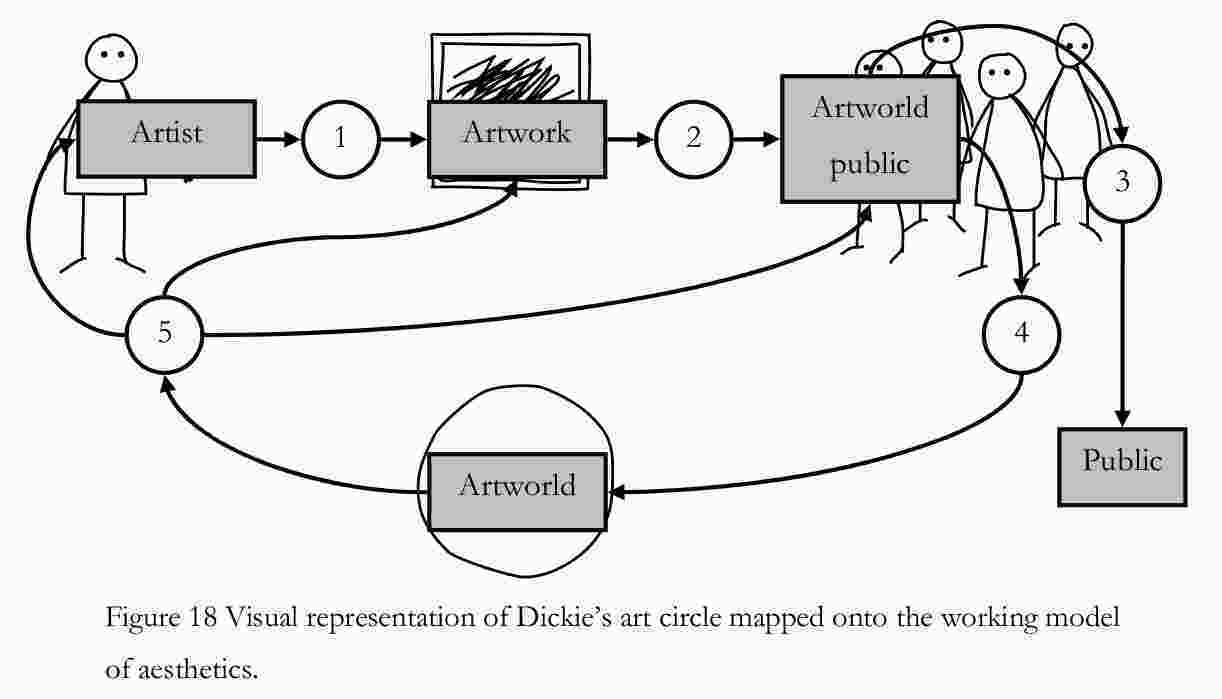
\includegraphics[width=\columnwidth]{./figures/artworld.jpg}

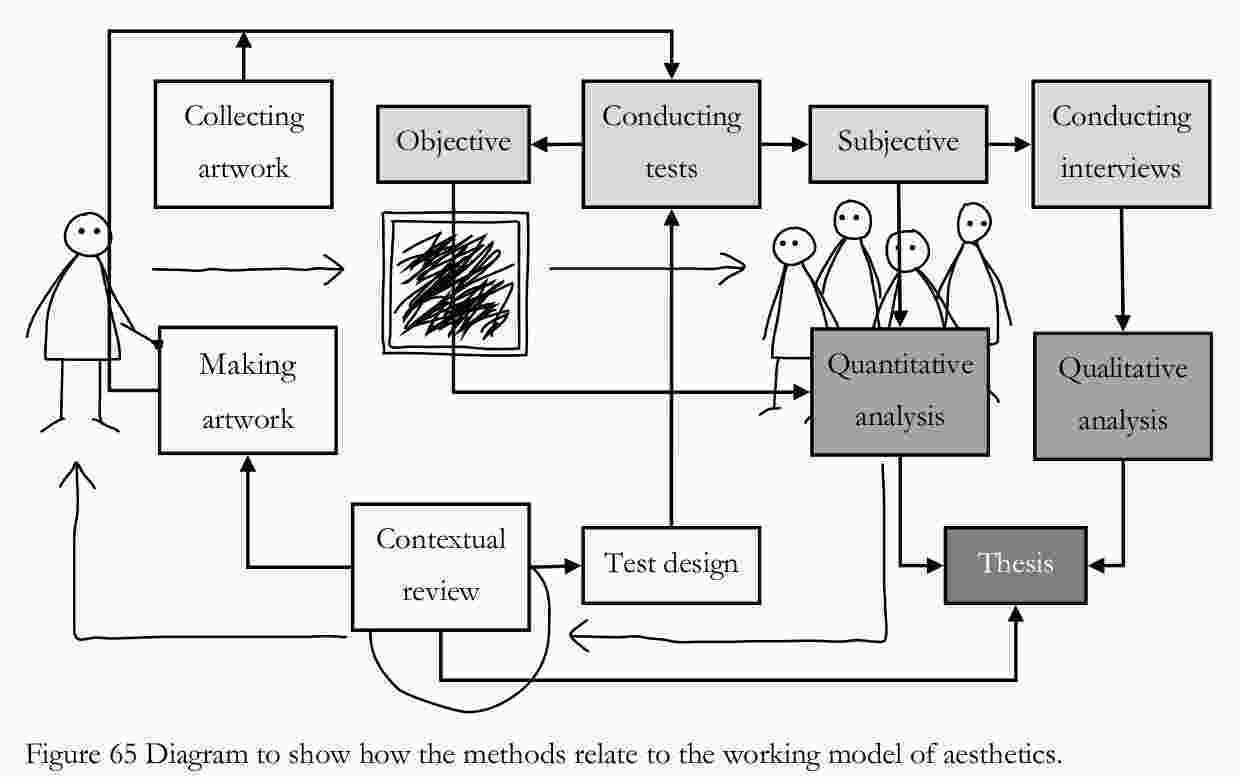
\includegraphics[width=\columnwidth]{./figures/aesthetic-research.jpg}

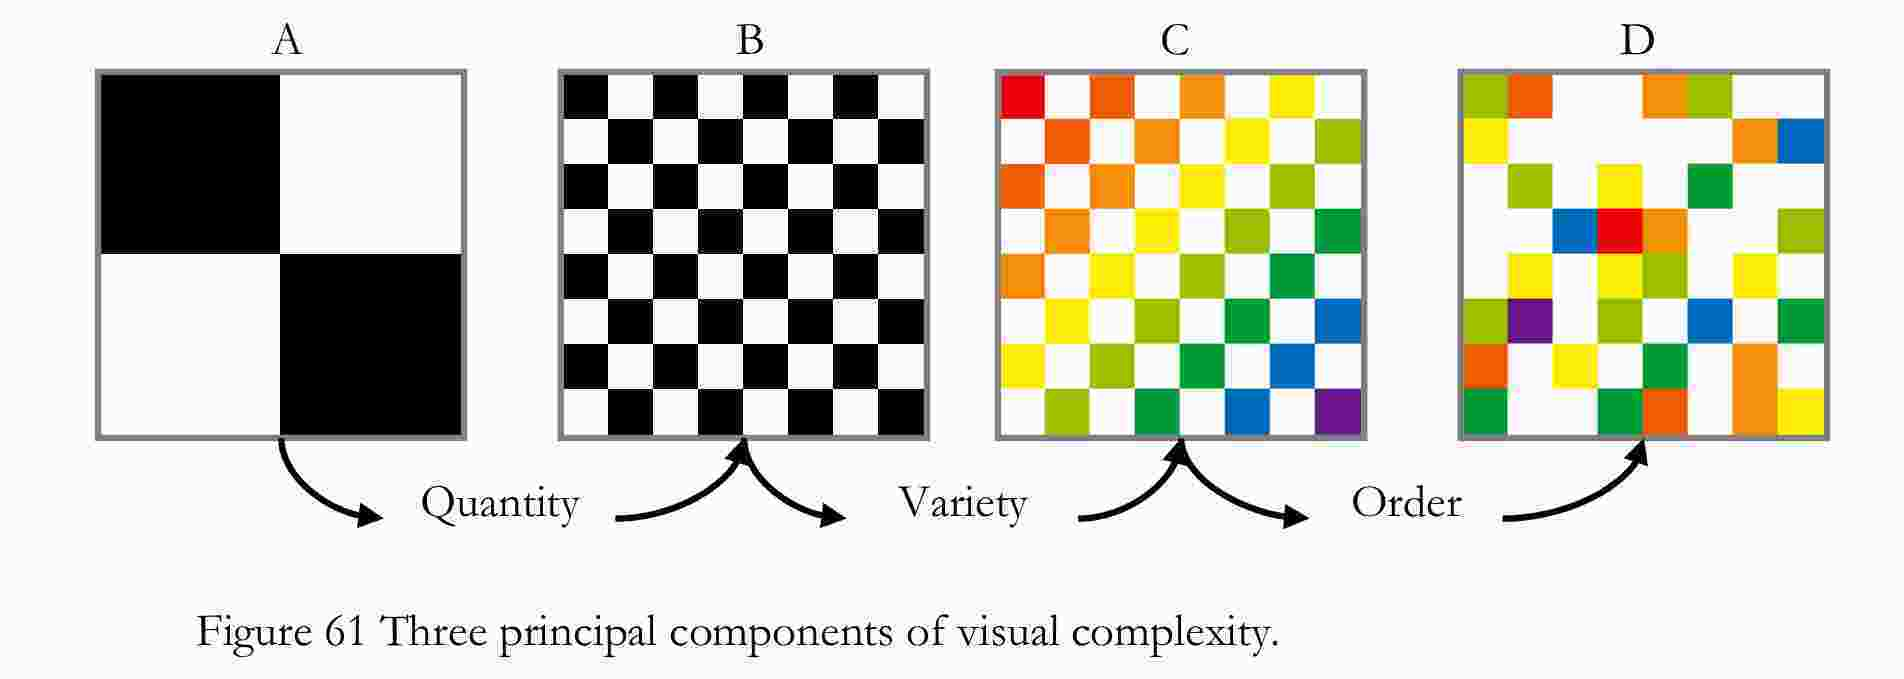
\includegraphics[width=\columnwidth]{./figures/quantity-variety-order.jpg}

%%COmment out 
%\bibliographystyle{apacite}
%\bibliography{./biblio}
%
%\end{document}


\bibliographystyle{apacite}
\bibliography{./biblio}

\end{document}
